%%
%% Author: shoupu_wan
%% 8/22/18
%%

\chapter{Case Study: Longest Palindrome Substrings}\label{ch:longestPalindromeSubstrings}

The longest palindrome substrings (LPS) in a given string has posed itself as an interesting
question.
It has also found widespread applications in mathematics, physics, chemistry, genetics, music,
\textit{etc.}
Here I pick it for two things.
First, to promote the conscious application of the study of symmetry to
understand and reduce a fairly complicated problem.
For any problem, identifying the hidden symmetry is the key to discover great
solutions to it.
Symmetry almost always brings saving and break of symmetry is almost always costly.
Secondly, we want to demonstrate how to apply the techniques explained earlier in this book,
particularly ~\autoref{prt:flowControl} and ~\autoref{prt:advancedTopic} to turn unreadable code
into more readable solution.
Let's jump to start.


\section{The problem Statement}\label{sec:lps-statement}

The problem statement of finding palindromic substrings take various forms in the literature.

For the sake argument, we state it as this:
\begin{quote}
    ``Given an input string, find the longest palindromic substring in it.
    Find the first if more than one exist.''
\end{quote}
According to Merriam-Webster dictionary, a palindrome is ``a word, phrase, or sequence that reads
the same backward as forward''.
Note that the length of a palindromic string can be odd or even and we can classify them as odd
palindrome and even palindrome, respectively.
For odd palindrome, its center of symmetry, or simply ``center'', falls on a
\code{char}.
For nonempty even palindrome, its center falls between two \code{char}s, which in this book
will be referred to as ``left center'' and ``right center'', respectively.
It becomes immediately obvious that there are a total of $2N+1$ palindromic substrings
in the input string and their centers include all the characters and boundaries between
adjacent characters.

To some programmers, merely solving the problem may not be ``hard'' so to speak.
For example, one may iterate through each possible center and for each center calculate the
length of LPS, searching successively for symmetric mismatches from center to brim.
The runtime complexity of such a supposed solution is no better than $O(N^2)$.
What is hard about this problem is to find a solution that beats the quadratic runtime.
In his paper in 1975, Glenn Manacher discovered a linear time solution to find the LPS that is a
prefix to a given string.
It was later found that his method works not only for the prefix but for all LPS's in the input
string.
This algorithm is the so-called \textit{the Manacher's algorithm}~\cite{Manacher:1975}.
We will dedicate some paragraph to understand this algorithm.
But first we need a little bit of math of symmetry as background information.


\section{Reflection symmetry}\label{sec:reflection-symmetry}

Reflection symmetry, \textit{a.k.a.}, mirror-image symmetry
\footnote{\url{https://en.wikipedia.org/wiki/Reflection_symmetry}} refers to space invariance
under reflection transformation.
A reflection transformation is the operation that transforms coordinates to their
mirror-image with respect to the fixed point, which we will refer as the ``axis of symmetry'' or
``center of symmetry''.
In one-dimensional ($1$D) space, a coordinate at $x$, its transformed coordinate $x^\prime$
\textit{w.r.t.} axis $a$ is:
\begin{equation}
    \label{eq:reflection-transform}
    x^\prime = 2a - x.
\end{equation}

\begin{figure}[H]
    \centering
    \caption{Two axes of reflection symmetry simultaneously present near each other will partition
    the entire space periodically and infinitely.
    Overlapping palindromes also form similar periodic patterns.}\label{fig:ReflectionSymmetry}
    \begin{subfigure}{.4\textwidth}
        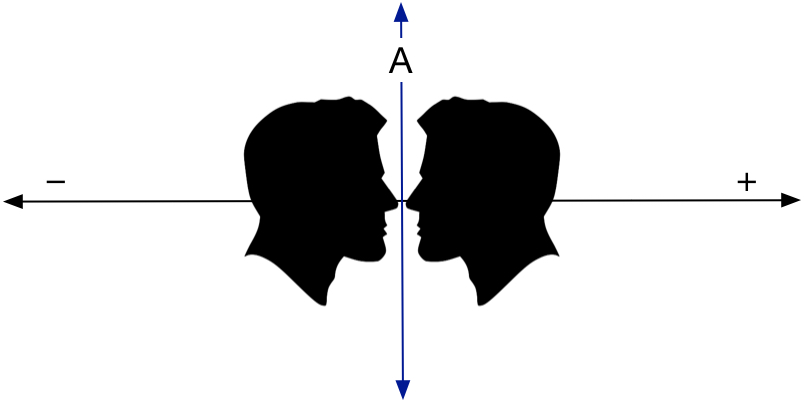
\includegraphics[width=\textwidth]{case-study/longest-palindrome/symmetry-axis-a.jpg}
        \caption{An axis of reflection symmetry}
        \label{fig:a-axis-reflection-symmetry}
    \end{subfigure}
    ~
    \begin{subfigure}{.4\textwidth}
        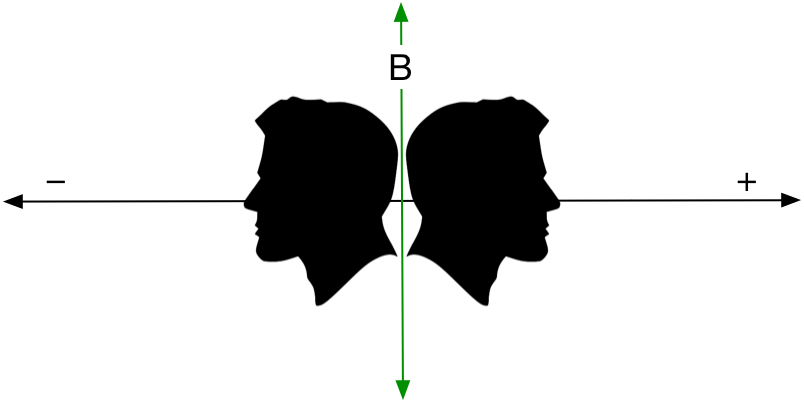
\includegraphics[width=\textwidth]{case-study/longest-palindrome/symmetry-axis-b.jpg}
        \caption{Another axis of symmetry}
        \label{fig:b-axis-reflection-symmetry}
    \end{subfigure}
    \vspace{1mm}
    \begin{subfigure}[b]{.4\textwidth}
        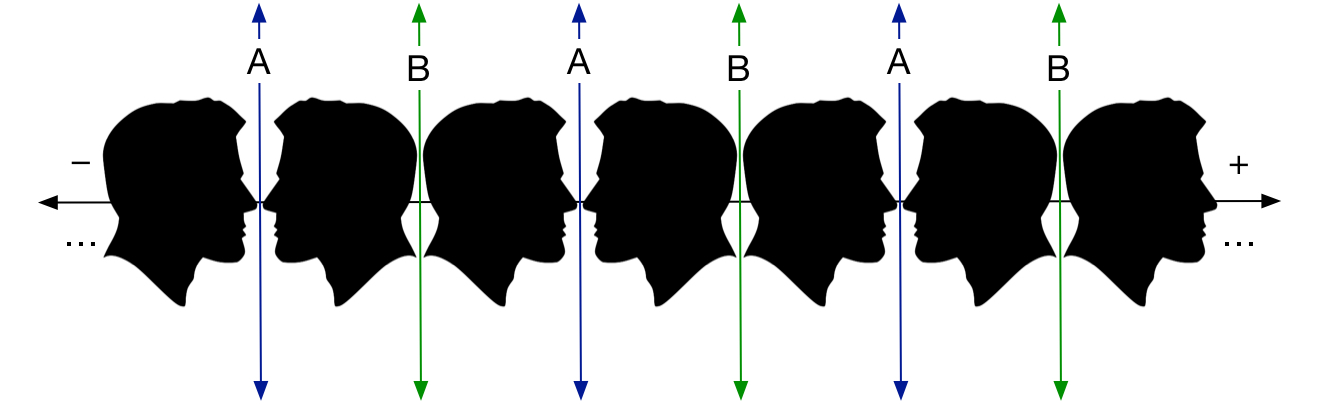
\includegraphics[width=\textwidth]{case-study/longest-palindrome/symmetry-2-axes.jpg}
        \caption{Two concurrent axes}
        \label{fig:two-axes-reflection-symmetry}
    \end{subfigure}
    ~
    \begin{subfigure}[b]{.4\textwidth}
        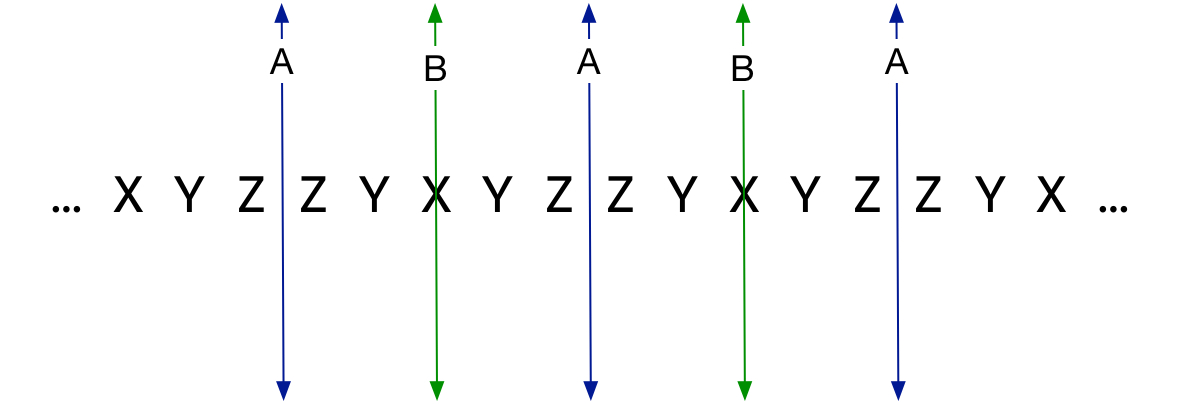
\includegraphics[width=\textwidth]{case-study/longest-palindrome/symmetry-palindrome.jpg}
        \caption{Overlapping palindromes}
        \label{fig:palindrome-symmetry}
    \end{subfigure}
\end{figure}

As shown in ~\autoref{fig:a-axis-reflection-symmetry}, axis of symmetry $A$ partitions the entire $1$D
space into left half-space and right half-space about itself, and points in the half-spaces have
one-to-one mapping.
Axis $B$ does similarly except \textit{w.r.t.} its own axis of symmetry
(\autoref{fig:b-axis-reflection-symmetry}).
If the two axes of reflection symmetry are simultaneously present along the $x$-axis, by
repetitively applying the reflection transformation, one may find infinitely many axes
periodically located along the $x$-axis and they partition the entire space into periodic regions
with period $2d$, where $d$ is the distance between the two axes of symmetry (see
~\autoref{fig:two-axes-reflection-symmetry}).
This effect may not be unfamiliar to
you if you have ever stepped in between two parallel mirrors---an array of clones of `you' appear,
alternately facing toward and away from you, aligned and coordinated.
This intuition of the multiple reflection symmetry is the key underlying the Manacher's algorithm.


\section{Problem Analysis}\label{sec:palindrome-problem-analysis}

Back to the LPS problem, we need to put it in the perspective of a discretized $1$D space.
The palindromic property of an infinite string manifest the reflection symmetry as shown in
~\autoref{fig:palindrome-symmetry}.
In reality, we do not have infinite space or string.
So the aforementioned symmetry may not be perfect.
Nevertheless as long as the regions of two reflection symmetry overlaps,
the above periodic argument still applies within the overlapping regions.
To facilitate coding and discussion, there are few special cases.
Firstly we treat the left and right end of the string as centers of zero length palindrome.
For empty string, the left and right ends collapse into one and that is the one and only
palindrome of the string.
All in all, for a string of length $n$, there are $(2 * n + 1)$ palindromic centers.
On each one of the centers, the longest palindrome can be found by extending the left and right
boundaries as far as the equally distant pairs of \code{char}s match.
It is interesting to consider the collective effect among these palindromic substrings.
The left and right wings of a palindromic string may host smaller palindromes.
When nearby palindromic substrings overlap, dwelling palindromes in the overlapping areas will be
mirrored to other parts of the string by symmetry,
When this happens, symmetric operations in the palindromic symmetry group may be
applied in again and again, in any combination by any order.
As a result, a substring $S$ may be mapped to mirror images $S^\prime$'s, images of images
$S^{\prime\prime}$'s, and so on.

\begin{figure}[htb]
    \centering
    \caption{\label{fig:bananas.palindrome}
    The top $4$ palindromic substrings of the example string ``bananas''
    labeled as `$1$`, `$2$`, and `$3$`.}
    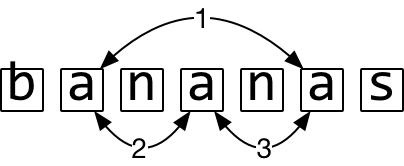
\includegraphics[width=.5\textwidth]{case-study/longest-palindrome/bananas-palindromes.jpg}
\end{figure}

\section{Manacher's algorithm}\label{sec:manacherAlgorithm}
%TODO
Manacher's algorithm is with memoir.
The key is to avoid repeated character comparisons.
Taking string ``bananas'' as an example, a few of its palindromic substrings are shown in
~\autoref{fig:bananas.palindrome}.
Note that these substrings overlap with one another.
Particularly, palindrome `$1$' tucks shorter palindromes `$2$', and
`$3$' under its left and right wings as we discussed in the previous section.
It's common practice that we iterate through the string from left to right and as one does so,
one caches the result, \textit{e.g.} the length as the following table shows.
\begin{center}
    \begin{tabular}{cccccccccccccccc}
        index:&0,&1,&2,&3,&4,&5,&6,&7,&8,&9,&10,&11,&12,&13,&14\\
        length:&0,&1,&0,&1,&0,&3,&0,&5,&0,&3,&0,&1,&0,&1,&0
    \end{tabular}
\end{center}
When examining a new center, the cached information for certain mirror image of it may be useful to
totally or partially determine the palindrome length.
For example, one can save on the calculation of the palindrome `$3$' by using the result of
palindrome `$2$'.

In one loop, there are two frontiers: center and checked char.
within the right wing as we scan down the centers.

\begin{alisting}[htb]
    \caption{\label{alg:lps-algorithm}
    Algorithm for calculating the length of LPS based on Manacher's algorithm}
    \begin{enumerate}
        \item Initialize an array \code{LPS} of size \code{2 * n + 1} and element at index \code{i}
        stores length of \code{LPS(i)}.
        \item Initialize \code{refCenter = 0}, which stores the palindrome center whose right wing
        reaches rightmost in each iteration of the main loop;
        \item For each \code{char} at \code{j = 0, 1, ..., n} in the augmented array,
        \begin{enumerate}[label={\roman*:}]
            \item If \code{j} lies to the right of the right wing of \code{PS(refCenter)},
            calculate \code{LPS(j)} from scratch;
            update \code{refCenter} accordingly;
            skip to the next iteration.
            \item Otherwise, find the mirror image of \code{j}
            with respect to \code{refCenter} and call it \code{jp}.
            \item If \code{LPS(jp)} is completely contained within \code{LPS(refCenter)}'s wing,
            then \code{LPS(j)=LPS(jp)};
            \item Otherwise (part of \code{LPS(j)} could pierce through
            the wing of \code{LPS(refCenter)}),
            then all we need is to calculate the exposed portion of \code{LPS(j)} to the right of
            \code{LPS(refCenter)}.
        \end{enumerate}
    \end{enumerate}
\end{alisting}

In some implementations, the original array is augmented by inserting
dummy \code{char}s in between each pair of neighboring \code{char}s in the original string and
require the palindrome substrings be centered on one of the \code{char} of the augmented string
(dummy \code{char} or original \code{char} alike).
So for \code{string} ``bananas'', the augmented array would be
\begin{figure}[h]
    \centering
    \caption{\label{fig:augmented-array-banana}
    Augmented array for \code{string} ``bananas''.
    The augmenting character chosen here is the blank space (ASCII 32).}
    \begin{center}
        \begin{tabular}{|c|c|c|c|c|c|c|c|c|c|c|c|c|c|c|}
            \hline
            \hline
            & b && a && n && a && n && a && s &\\
            \hline
            \hline
        \end{tabular}
    \end{center}
\end{figure}

Then all the palindromic substrings are centered on one of the \code{char} in the augmented
string for sake of implementation.
Algorithm is outlined in ~\autoref{alg:lps-algorithm}.


\section{Augmented-String Implementations}\label{sec:implementation-lps-augmented}

With the background information and outline of the algorithm in ~\autoref{alg:lps-algorithm},
it is straightforward to implement Manacher's algorithm literally following the algorithm.
In fact several implementations may be found on the Internet.
A \java version by CS department of Princeton
University\footnote{\url{https://algs4.cs.princeton.edu/53substring/Manacher.java.html}},
A \python version by Fred Akalin\footnote{\url{https://www.akalin .com/longest-palindrome-linear-time}},
An explanation of the algorithm and a Haskell
implementation in Johan Jeuring's blog\footnote{
\url{http://finding-palindromes.blogspot.com/2012/05/finding-palindromes-efficiently.html}},
along with others.
An implementation of my own is also provided here for sake of argument and reference
(~\autoref{lst:LongestPalindromeAugment}).
(For comparison purposes, all the implementations made in this chapter are in \java.)

\newpage
\begin{clisting}[H]
    \lstinputlisting[label={lst:LongestPalindromeAugment},language=Java,escapechar=~,
    caption={A implementation of Manacher's algorithm for the LPS problem.
    Original string is literally augmented in memory.}]
    {case-study/longest-palindrome/LongestPalindromeAugment.java}
\end{clisting}


\section{Virtual mapping for augmented string}\label{sec:virtualMapping}

The string-augmentation process in ~\autoref{lst:LongestPalindromeAugment} is not
only tedious and costly in memory footprint, it also demands the identification of
an augmenting character that is absent from the original string to avoid spurious result.
In this section, we seek to find a more concise and economic way to
implement Manacher's algorithm.
The idea is based on index mapping between the original and augmented strings.


\begin{savenotes}
    \begin{table}[htb]
        \centering
        \caption{\label{tab:semantics-arithmetic} Semantics of index arithmetic expressions given
        \code{i} being the palindromic center and \code{x} an arbitrary index, both in the augmented
        string; \code{lps} is the array storing lengths of palindromic substrings.}
        %        \vskip 10pt
        \begin{tabular}{l|l}
            \hline
            Arithmetic & Semantic\\
            \hline
            \code{i / 2} & The left center in the original string.
            meaningful only for even \code{i}\\
            \code{(i - 1) / 2} & The center in the original string.
            meaningful only for odd \code{i}\\
            \code{2 * i - x} & mirror index of \code{x} about the center \\
            \code{i - lps[i]} & left bounding index of the palindromic substring\\
            \code{i + lps[i]} & right bounding index of the palindromic substring \\
            \code{(i - lps[i]) / 2} & left index mapped to the original string \footnote{
            \label{odd-odd-even-even} This is because if center is even, length of the
            palindromic substring around this center can only be even.
            Conversely, if center is odd, length of the palindromic substring
            around this center can only be odd} \\
            \code{(i + lps[i]) / 2} & right index mapped to the original string
            \textsuperscript{\ref{odd-odd-even-even}} \\
            \hline
        \end{tabular}
    \end{table}
\end{savenotes}


Consider the string ``bananas'' (~\autoref{fig:bananas.palindrome}) and its augmented string as
shown in ~\autoref{fig:augmented-array-banana}, there is a $1:1$ correspondence between the
indexes in the original and the augmented strings.
Arithmetic expressions with certain semantic meaning has been created in
table ~\autoref{tab:semantics-arithmetic}.


By extensively using index arithmetic, one can simulate a `virtualized augmentation' of the
original string without actually constructing the augmented string in memory.
It helps reduce memory footprint and also free us from the burden of choosing a dummy character.
Following closely to what has been discussed, we implemented the `virtual augmentation' as
shown in ~\autoref{lst:LongestPalindrome}.
Implementation ~\autoref{lst:LongestPalindrome} has $O(N)$ complexity for both runtime memory.
So far, it is one of the most performant implementations known.

\newpage
\begin{clisting}[H]
    \lstinputlisting[label={lst:LongestPalindrome},language=Java,escapechar=~,
    caption={Implementation of Manacher's aglorithm using index mapping.}]
    {case-study/longest-palindrome/LongestPalindromeIndexMapping.java}
\end{clisting}

\section{Solutions for Readability}\label{sec:palindrom.modularized}

The virtual mapping frees us from actually augmenting the input string and proves a great
solution with both optimal runtime complexity and optimal memory footprint.
But looking at the code in ~\autoref{lst:LongestPalindrome}, it is far from clean or compact.
In fact it is quite unreadable.
This is because there are full of arithmetic expressions for symmetry transformations, key look
ups, \textit{etc.}
These arithmetic mappings degrade its readability quite a bit.


How can go about making it more readable?
The key is two-fold.
First, reduce duplicate code.
If you look carefully, there are quite a few occurrences of soft duplication.
Secondly, refactor the monolithic implementation into succinct, meaningful helper functions.
This goal is correlated with the first in that some of the helper functions may be reused to
reduce duplicate code.
Let us start with ~\autoref{lst:LongestPalindrome} and use it to demonstrate
how to apply techniques discussed in this book to achieve our goal.

First, observe that the code is bloated with duplicate code.
For example, a pattern is repeated on line ~\autoref{line:lps-soft-duplication}:
\begin{lstlisting}
    if (im - lps[im] > maxi - lps[maxi])
\end{lstlisting}
It may be obscure to untrained eyes.
But the pattern is clear---given an index, get the index minus the element
at the index as the result.
So we can factor that out into a function and get rid of the duplication.
What name should we give the function?
Well, what's being returned?

\lstinputlisting[label={lst:lpsModuler},firstline=3,language=Java,escapechar=~,
caption={Java implementation of longest
palindrome substring Manacher's aglorithm.}]
{case-study/longest-palindrome/LongestPalindromeModular.java}


\section{Conclusion}\label{sec:conclusion}
%TODO
